\chapter{Cinta de Möbius de paper òptima}
{\color{blue}La idea d'aquest capítol és la següent:
\begin{itemize}
    \item Introduir que estem parlant d'això per mostrar d'una altra manera la rigidesa dels encabiments suaus.
    \item Explicar el problema de la cinta de Möbius de paper òptima.
    \item Enunciar i demostrar el teorema principal.
    \item Enunciar i demostrar el teorema del límit triangular.
    \item Explicar l'acordió de Möbius, donant peu al següent capítol.
\end{itemize}
}
\section{Introducció al capítol}
Al capítol anterior hem vist que, tot i que sempre existeix algun espai euclidià de dimensió prou alta tal que s'hi pugui encabir una varietat topològica $C^\infty$, pel teorema de Whitney, no sempre és possible encabir-los en espai de dimensió 3. En concret, fins i tot per varietats que sí es poden encabir suaument en $\mathbb R^3$, hem vist que no sempre és possible encabir-les isomètricament, com hem vist en el cas del tor. 

A continuació presentem un resultat obtingut recentment, l'any 2023, per Richard Evan Schwartz, on demostra una altra restricció per una varietat amb frontera, aquesta vegada en el cas de les cintes de Möbius. Veurem que, tot i que és possible encabir-les suaument i isomètrica en $\mathbb R^3$ quan el costat llarg de la cinta de Möbius és $\sqrt3$ vegades major que el curt, no és possible fer-ho quan és més petit. 

L'objectiu d'aquest capítol no serà només veure aquest resultat, sinó també veure com el podem "esquivar" relaxant les condicions del nostre encabiment isomètric. La manera en què ho aconseguirem apuntarà cap al que veurem al capítol següent, on demostrarem el teorema de Nash. 

La font d'aquest capítol és gairebé exclusivament la versió més nova de l'article de Richard Evan Schwartz, \cite{schwartz2024}. Aquest article és molt senzill, curt i fàcil de llegir, de manera que seguim de manera molt propera la seva demostració. Hem afegit els diagrames de la demostració del lema T per tal de fer més evident l'argument topològic que fa servir Schwartz.

{\color{red} El Schwartz menciona aquí uns papers que expliquem més sobre la banda de Möbius, si volem escriure més sobre el tema els podem utilitzar.}

\section{Introducció al problema}

\subsection{Definicions}
\begin{defi}
    Anomenem \textbf{cinta de Möbius plana de raó d'aspecte $\lambda$} la varietat topològica amb frontera {\color{blue} Hem de definir a la secció anterior varietat topològica amb frontera} obtinguda amb la següent identificació d'un rectangle
    $$M_\lambda := ([0,\lambda] \times [0,1])/\sim, \quad\quad (0,y)\sim(\lambda,1-y).$$
\end{defi}

\begin{defi}
    Una \textbf{cinta de Möbius de paper de raó d'aspecte $\lambda$} és una aplicació isomètrica $I:M_{\lambda}\to\mathbb R^3$ de classe $C^\infty$
\end{defi}
\begin{nota}
    Anomenarem $\Omega=I(M_\lambda)$ la imatge de $M_\lambda$ per $I$. Quan $I$ sigui un encabiment, direm que $\Omega$ està \textbf{encabida} en $\mathbb R^3$.
\end{nota}

\begin{ex}
    Anomenem \textbf{cinta de Möbius de paper triangular} la cinta de Möbius de paper de raó d'aspecte $\lambda = \sqrt{3}$.
\end{ex}

\subsection{Enunciats dels teoremes}
\begin{teo}[\textbf{Principal}]\label{teo:Main Schwartz}
    Una cinta de Möbius de paper encabida en $\mathbb R^3$ té raó d'aspecte més gran que $\sqrt{3}$.
\end{teo}

{\color{red} AIXÒ IMPORTA? SI SOBRA ESPAI ENS HO PODEM CARREGAR}
\begin{teo}[\textbf{Límit Triangular}]\label{teo:Límit triangular}
    Sigui $I_n:M_{\lambda_n}\to\mathbb R^3$ una successió de cintes de Möbius de paper suaus encabides, tals que $\lambda_n\to\sqrt{3}$. Aleshores, $I_n$ convergeix uniformement a una cinta de Möbius de paper triangular, llevat d'isometria.
\end{teo}

\subsection{Preliminars a la demostració}
\begin{defi}
    Sigui $I:M_\lambda\to\Omega$ una cinta de Möbius de paper encabida. Un \textbf{plec} a $\Omega$ és un segment de recta $B'$ que talla a través de $\Omega$ i té els seus extrems a la frontera.
\end{defi}

\begin{defi}
    Sigui $B'$ un plec. Anomenem \textbf{pre-plec} a la preimatge $B=I^{-1}(B')$.
\end{defi}
Veurem més endavant que tota cinta de Möbius de paper encabida té una foliació per plecs. A més, degut al fet que $I$ no incrementa distàncies, és fàcil veure que els pre-plecs també són segments de recta, i que $M_\lambda$ té una foliació per pre-plecs. {\color{blue} Hem de definir foliació preferiblement.}
\begin{defi}
    Un \textbf{patró T en $\Omega$} (en anglès, \textit{T-pattern}) és un parell de plecs que es troben en rectes perpendiculars que intersequen en un punt. Diem que el patró T està \textbf{encabit} en $\Omega$ si els plecs no intersequen.
\end{defi}

El Teorema Principal es desprendrà de la demostració dels dos lemes que enunciem a continuació.
\begin{lema}[\textbf{T}]\label{lema T}
    Tota cinta de Möbius de paper encabida té un patró T encabit.
\end{lema}

\begin{lema}[\textbf{G}]\label{lema G}
    Tota cinta de Möbius de paper encabida amb un patró T encabit té raó d'aspecte més gran que $\sqrt{3}$.
\end{lema}

\section{Demostració}
\subsection{Existència de la foliació per plecs}
Sigui $\Omega^\circ$ l'interior de $\Omega$, i $U$ el subconjunt de $\Omega^\circ$ format pels punts té curvatura mitjana {\color{blue} Hem de definir curvatura mitjana!!!} diferent de zero.

Per demostrar l'existència de la foliació per plecs, utilitzarem el lema següent:
\begin{lema}\label{lema:2.2}
    Tot punt $p\in U$ pertany a un únic plec $\gamma$, i tot punt de $\gamma$ té curvatura mitjana diferent de zero, fins i tot a la frontera. {\color{blue} hauríem de mirar de demostrar això si és possible.}
\end{lema}

\begin{teo}[\textbf{Existència de la foliació per plecs}]
    $\Omega$ té una foliació per plecs.
\end{teo}
{
    \color{green!50!black}
    \textit{Prova.}
    Sigui $U^*$ la unió de tots els plecs que passen per punts de $U$. Observem que els punts de la frontera de cada plec pertanyen a $U^*$. Els punts de $U^*$ no intersequen, ja que altrament aquell punt tindria curvatura mitjana zero, contradient el lema \ref{lema:2.2}. Per tant, $U^*$ té una foliació per plecs. 

    Sigui $\tau'$ un component connex de $\Omega\setminus U^*$.
    Si $\tau'$ té interior buit, aleshores és el límit d'una successió de plecs de $U^*$, i per tant és també un plec en ser un segment de recta.
    Si $\tau'$ té punts al seu interior, aleshores tots ells tenen curvatura mitjana zero, de manera que pertanyen a un sol pla.
    Sigui $\tau = I^{-1}(\tau')$. $I|_{\tau}$ és un encabiment isomètric entre regions planes i $\tau$ és un trapezoide convex. Per tant, $I|_{\tau}$ és una isometria global, de manera que les imatges de segments de recta en $\tau$ són segments de recta. Podem obtenir una foliació per pre-plecs de $\tau$ de manera senzilla interpolant entre els dos pre-plecs de la seva frontera, i prendre la imatge per $I$ d'aquesta foliació per obtenir una foliació per plecs de $\tau'$.{\color{blue} Podem posar un dibuixet tranquilament, tinc un de molt maco a la pàgina 2 dels apunts.}

    Realitzant aquest procés per cada component connex de $\Omega\setminus U^*$, obtenim una foliació per plecs de $\Omega$.
    \qed
}
\subsection{Demostració del lema T}
\begin{defi}
    Sigui $I:M_\lambda\to\Omega$ una cinta de Möbius de paper encabida. 
    Anomenem \textbf{línia central de $M_\lambda$} al cercle $([0,\lambda]\times\set{1/2})/\sim$.
    Anomenem \textbf{línia central de $\Omega$} a la imatge de la línia central de $M_\lambda$ per $I$.
\end{defi}

\begin{defi}
    Sigui $u$ un plec. Anomenem \textbf{orientació de $u$} a cada un dels dos vectors unitaris paral·lels a $u$, $\pm \vec u$.
\end{defi}

\begin{prop}
    Tot pre-plec interseca la línia central de $M_\lambda$ en un únic punt.
\end{prop}
{
    \color{green!50!black}
    \textit{Prova.}
    Sigui $u$ un pre-plec, i $\ell(u)$ la seva longitud. Si $\ell(u)<\sqrt{1+\lambda^2}$, es pot desplaçar per una isometria per tal que no toqui les verticals del rectangle, de manera que clarament ha de tallar a la línia central en un únic punt.
    Suposem, per tant, que $\ell(u)\geq\sqrt{1+\lambda^2}$. Aleshores, $\ell(u)>\lambda$. Però la frontera $\partial \Omega$ és un cercle (topològic) de longitud $2\lambda$ que conté els extrems del plec $I(u)$. Per tant, $2\lambda = \ell(\partial \Omega) \ge  2\ell(I(u)) = 2\ell(u)>2\lambda$, que és una contradicció.
    \qed
}
\begin{obs}
    Escollint una foliació per plecs $\beta$, el fet que $I$ és un encabiment implica que la proposició també és certa per plecs: tot plec interseca la línia central de $\Omega$ en un únic punt. Així, podem associar a cada plec de $\beta$ un únic valor de $\mathbb R/2\pi$
\end{obs}

Sigui $\Gamma$ l'espai de parelles $(x_0,x_1)\in(\mathbb R/2\pi)^2$ tals que $x_0\neq x_1$. Per la observació anterior, cada parella de plecs de $\beta$ diferents es correspon amb un únic element de $\Gamma$. $\Gamma$ és homeomorf a un cilindre.

Podem compactificar $\Gamma$ afegint $\partial_+$ com el límit de les parelles en què $x_1$ va just abans que $x_0$ en el cilindre, i $\partial_-$ com el límit de les parelles en què $x_1$ va just després que $x_0$. Aquest nou espai, $\overline{\Gamma}$, és homeomorf a l'esfera $\mathbb S^2$. L'aplicació $\Sigma(x_0,x_1) = (x_0,x_1)$ es pot estendre a una aplicació contínua de l'esfera que bescanvia $\partial_+$ i $\partial_-$.
{\color{blue} DIBUIXET!!!}

Per tot parell $(x_0,x_1)\in{\Gamma}$, hi ha un únic camí positiu $\set{x_t}$ en l'ordre cíclic de $\mathbb R/2\pi$ que va de $x_0$ a $x_1$. Aquest camí té longitud propera a zero quan $(x_0,x_1)$ està a prop de $\partial_+$, i propera a $2\pi$ quan $(x_0,x_1)$ està a prop de $\partial_-$.

Escrivim $\vec u_0\rightsquigarrow\vec u_1$ per denotar que hi ha una orientació contínua de plecs $\set{u_t}$ amb extrems $u_0$ i $u_1$. Notem que, si $\vec u_0\rightsquigarrow\vec u_1$, aleshores $-\vec u_0\rightsquigarrow-\vec u_1$, ja que és un canvi d'orientació, i que $\vec u_1\rightsquigarrow-\vec u_0$, ja que ens trobem en una cinta de Möbius. 

Sigui $m_j$ el punt mig de $u_j$. Definim l'aplicació
\begin{align*}
    F=(g,h): {\Gamma}&\to\mathbb R^2,\\
    (x_0,x_1)&\mapsto(\vec u_0\cdot\vec u_1, (m_0- m_1)\cdot(\vec u_0\times\vec u_1))
\end{align*}
on $\vec u_0\rightsquigarrow\vec u_1$. Notem que la definició és independent de la orientació, ja que $\vec u_0\rightsquigarrow\vec u_1\iff-\vec u_0\rightsquigarrow-\vec u_1$, i que $F$ es pot estendre de manera contínua a $\mathbb S^2$ de la següent manera:
\begin{align*}
    \overline{F}=(\overline{g},\overline{h}): \overline{\Gamma}&\to\mathbb R^2,\\
    (x_0,x_1)&\mapsto\begin{cases}
        F(x_0,x_1) & \text{si } (x_0,x_1)\in{\Gamma},\\
        (\pm 1,0) & \text{si } (x_0,x_1)={\partial_\pm}.
    \end{cases}
\end{align*}

\begin{prop}
    $F$, tal com l'hem definit, és tal que $F\circ\Sigma = -F$.
\end{prop}
{
    \color{green!50!black}
    \textit{Prova.}
    Només cal veure que és cert per les funcions $g$ i $h$. Utilitzem que $\vec u_0\rightsquigarrow\vec u_1\iff-\vec u_0\rightsquigarrow-\vec u_1$.

    Com $g(x_0,x_1) = \vec u_0\cdot\vec u_1$, tenim que $g(x_1,x_0) = \vec u_1 \cdot (-\vec u_0) = -g(x_0,x_1)$.

    Com $h(x_0,x_1) = (m_0- m_1)\cdot(\vec u_0\times\vec u_1)$, tenim que $h(x_1,x_0) = (m_1- m_0)\cdot(\vec u_1\times(-\vec u_0)) = (m_1- m_0)\cdot(\vec u_0\times\vec u_1) = -h(x_0,x_1)$.
    \qed
}

A més, pels punts antipodals $\partial_+$ i $\partial_-$ tenim que $\overline{F}(\partial_+) = \overline{F}(\partial_-) = (1,0)$.

Com $\overline{F}$ és contínua una aplicació contínua sobre un domini homeomorf a una esfera tal que $\overline{F}\circ\Sigma = -\overline{F}$, pel teorema de Borsuk-Ulam, existeix algun punt del domini amb imatge nul·la. Aquest punt no pot ser $\partial_+$ ni $\partial_-$, ja que $\overline{F}(\partial_\pm) = (\pm1,0)$, per tant ha de pertànyer a $\Gamma$.

Siguin $(u_0,u_1)$ els plecs corresponents a $(x_0,x_1)\in F^{-1}(0,0)$.
Aleshores:
\begin{enumerate}
    \item $u_0$ i $u_1$ són disjunts, ja que són plecs diferents d'una mateixa foliació.
    \item $u_0$ i $u_1$ són ortogonals, ja que $g(x_0,x_1) = 0$.
    \item $u_0$ i $u_1$ són coplanars, ja que $h(x_0,x_1) = 0\implies$ $\vec u_0$, $\vec u_1$ i $m_0-m_1$ són tots ortogonals a $\vec u_0\times\vec u_1$.
\end{enumerate}

Tot plegat, implica que $u_0$ i $u_1$ formen un patró T encabit, com volíem demostrar.

\subsection{Demostració del lema G}
\begin{nota}
    Sigui $\ell$ la longitud d'arc, $\triangledown$ un triangle de base horitzontal i $\lor$ els costats no-horitzontals.
\end{nota}

\begin{defi}
    Si $\triangledown$ té base $\sqrt{1+t^2}$ i alçada $h\ge1$, aleshores $\ell(\lor)\ge\sqrt{5+t^2}$. La igualtat es compleix si i només si $h=1$ i $\triangledown$ és isòsceles.
\end{defi}

{
    \color{green!50!black}
    \textit{Prova.}
    Siguin $p_1$, $p_2$ i $q$ els vèrtexs de $\triangledown$, amb $p_1p_2$ la base. Sigui $p_2'$ el simètric de $p_2$ respecte de la recta horitzontal que passa per $q$. Aleshores,
    \begin{equation*}
        \ell(\lor) = \|p_1-q\| + \|p_2-q\| = \|p_1-q\| + \|p_2'-q\| \ge \|p_1-p_2'\| = \sqrt{1+t^2+4h^2}\ge\sqrt{5+t^2}.
    \end{equation*}
    La igualtat es compleix si i només si $h=1$ i $p_1p_2'$ és vertical, que és el cas de l'isòsceles.
    \qed
}

Sigui $I:M_\lambda\to\Omega$ una cinta de Möbius de paper encabida amb un patró T encabit.
\begin{nota}
    Per qualsevol subconjunt $S\subseteq M_\lambda$, anomenem $S'=I(S)$ la imatge de $S$ per $I$.
\end{nota}

Rotem $\Omega$ tal que un plec sigui horitzontal, $T'$, i l'altre estigui per sota en el mateix pla, $B'$. Observant $\Omega$ i $M_\lambda$, verifiquem que tenen la forma de la figura {\color{red} DIBUIXET!!!}

Ara observem que 
\begin{equation*}
    \begin{cases}
        \text{base} &= \ell(T') = \ell(T) = \sqrt{1+t^2},\\
        \text{alçada} &> \ell(B') = \ell(B) = \sqrt{1+b^2}\ge1.
    \end{cases}
\end{equation*}

Per tant, es verifiquen
\begin{equation*}
    \begin{cases}
        \ell(H) + \ell(D) = 2\lambda\\
        \ell(D)-2t=\ell(H)\\
        \sqrt{1+t^2}=\ell(T')\le\ell(H')=\ell(H)\\
        \sqrt{5+t^2}<\ell(\lor)\le\ell(D')=\ell(D)
    \end{cases}
\end{equation*}

Definim les corbes
\begin{equation*}
    \begin{cases}
        \alpha(t) := \sqrt{1+t^2} + \sqrt{5+t^2}<\ell(H) + \ell(D) = 2\lambda\\
        \beta(t) := 2\sqrt{5+t^2}-2t < 2\ell(D)-2t = \ell(D) + \ell(H) = 2\lambda
    \end{cases}
\end{equation*}

Per tant, $2\lambda > \max(\alpha(t),\beta(t))$. Posant $t_0 = 1/\sqrt{3}$, tenim que $\alpha(t_0) = \beta(t_0) = 2\sqrt3$.

Observem que $\alpha$ és creixent en $(0,\infty)$. Per tant, $\alpha(t)>2\sqrt3$ per a tot $t>t_0$. En canvi, $\beta$ és decreixent en $t\in\mathbb R$. Per tant, $\beta(t)>2\sqrt3$ per a tot $t<t_0$. Tot plegat, obtenim que $\lambda>\sqrt3$, com volíem demostrar.


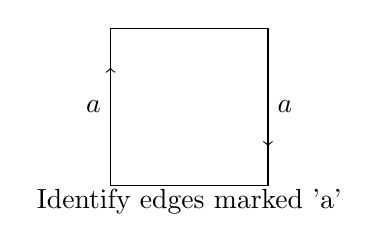
\begin{tikzpicture}
    \draw (0,0) rectangle (2,2); % Draws a square
    \draw[->] (0,0.5) -- (0,1.5) node[left, midway] {$a$}; % Arrow on left edge
    \draw[->] (2,1.5) -- (2,0.5) node[right, midway] {$a$}; % Arrow on right edge (Mobius identification)
    \node at (1,-0.2) {Identify edges marked 'a'};
  \end{tikzpicture}



\newpage